\documentclass[10pt]{article}
\usepackage{amsmath,amssymb,epsfig,graphics,hyperref,amsthm,mathtools,
  mdframed,enumitem}
\DeclarePairedDelimiter\ceil{\lceil}{\rceil}
\DeclarePairedDelimiter\floor{\lfloor}{\rfloor}

\hypersetup{colorlinks=true}

\setlength{\textwidth}{7in}
\setlength{\topmargin}{-0.575in}
\setlength{\textheight}{9.25in}
\setlength{\oddsidemargin}{-.25in}
\setlength{\evensidemargin}{-.25in}

\reversemarginpar
\setlength{\marginparsep}{-15mm}

\newcommand{\rmv}[1]{}
\newcommand{\bemph}[1]{{\bfseries\itshape#1}}
\newcommand{\N}{\mathbb{N}}
\newcommand{\Z}{\mathbb{Z}}
\newcommand{\imply}{\to}
\newcommand{\bic}{\leftrightarrow}

% Some user defined strings for the homework assignment
%
\def\Author{Shuo Yang}

\begin{document}

\noindent

% \CourseCode \hfill \DateHandedOut

\begin{center}
  Experiment results\\
  Shuo Yang\\
  \vspace{1em}
\end{center}

% A horizontal split line
\hrule\smallskip
\vspace{1em}
\underline{\textbf{Experiment setup}}\\

Topology: dumbbell topology as shown in the below figure:

\begin{center}
  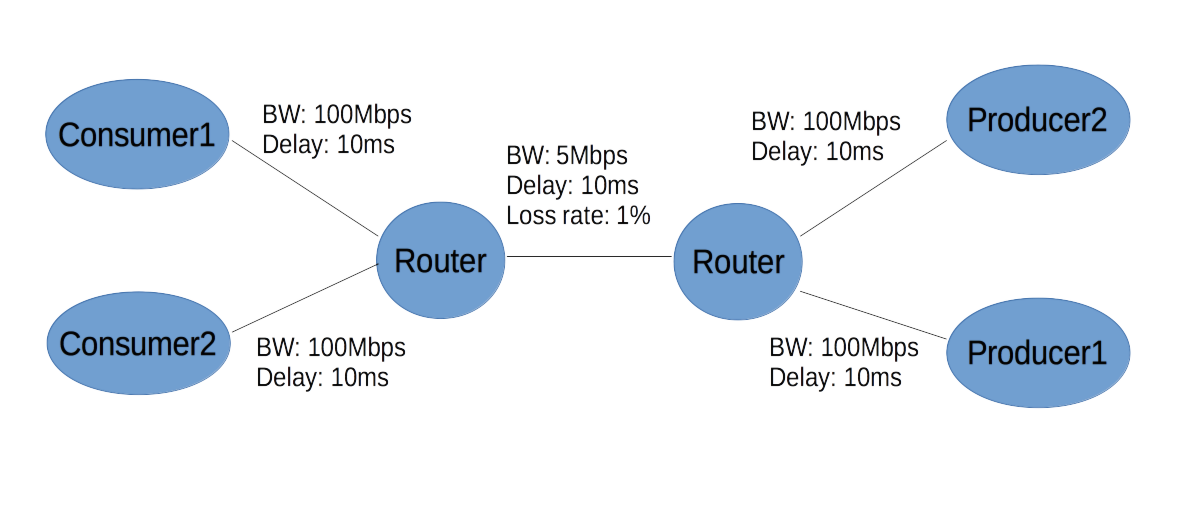
\includegraphics[width=14cm,height=6cm]{./dumbbell.png}
\end{center}

Traffic: cross traffic (consumer1 downloads file from producer1 and
consumer2 downloads file from producer2).\\

Bottleneck link: the link between 2 routers with bandwidth of 5Mbps,
delay of 10ms and loss rate as 1\%. All other links all have bandwidth
of 100Mbps and delay of 10ms.\\

File size: 10MB.\\

Segment size: 1024 byte\\

Simulation platform: Mini-ndn.\\

Metrics:

\emph{Download time}: total time (in seconds) it takes to download the file.

\emph{Throughput}: calculated as (total number of data packets received *
data packet size) / (total download time).

\emph{Loss rate}: calculated as (total number of retransmitted packets) /
(total number of packets received).

\emph{congestion window size}: measured every 200ms

\emph{RTT and RTO}: measured every time a data packet was received (not
including those retransmitted ones)\\

Consumer implementations: one implements AIMD (to mimic TCP tahoe) and
the other one implements AIMD + sequence hole detection (to mimic TCP
reno). In the following I will use \emph{aimd} to refer to the first
implementation and \emph{reno} to refer to the second implementation.\\

\underline{\textbf{Results}}\\

\begin{tabular}{ | l | l | l | l |}
  \hline
  & download time & throughput & loss rate \\\hline
  aimd & 52s & 1605 Kbps & 2.1\% \\\hline
  reno & 62s & 1347 Kbps & 2.2\% \\\hline
\end{tabular}

\vspace{1em}

The figure below shows how congestion window changes over time in the
\emph{aimd} implementation:

\begin{center}
  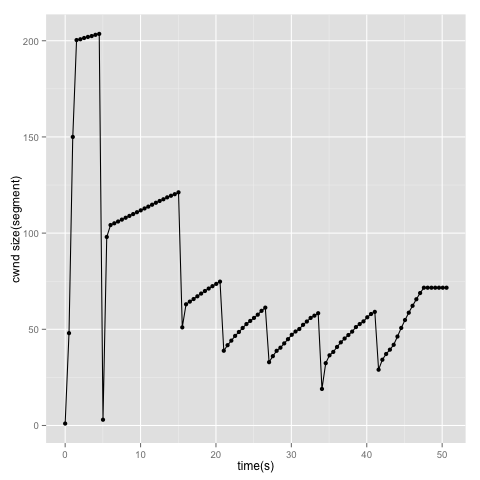
\includegraphics[width=10cm,height=8cm]{./cwnd_aimd.png}
\end{center}

The figure below shows how measured RTT and RTO change over time in
the \emph{aimd} implementation:

\begin{center}
  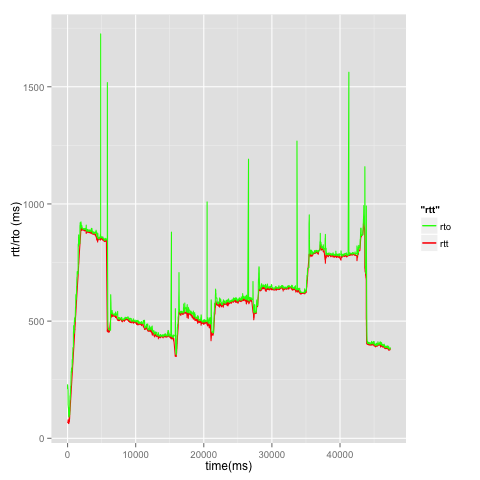
\includegraphics[width=10cm,height=8cm]{./rttrto_aimd.png}
\end{center}

The figure below shows how congestion window changes over time in the
\emph{reno} implementation:

\begin{center}
  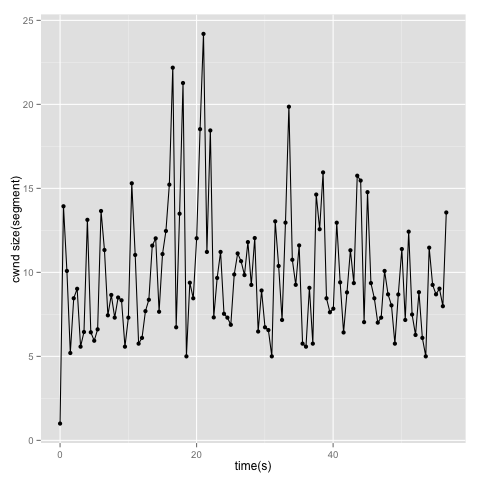
\includegraphics[width=10cm,height=8cm]{./cwnd_reno.png}
\end{center}

The figure below shows how measured RTT and RTO change over time in
the \emph{reno} implementation:

\begin{center}
  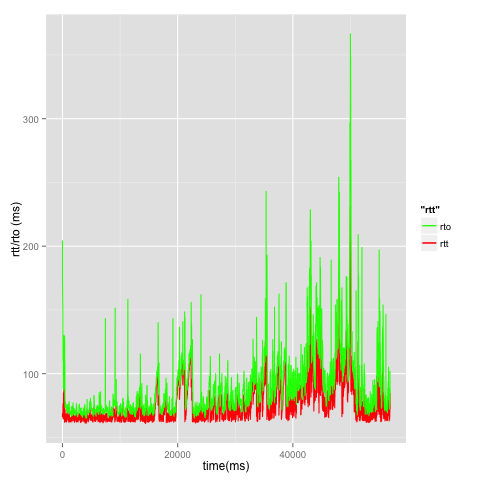
\includegraphics[width=10cm,height=8cm]{./rttrto_reno.png}
\end{center}

\underline{\textbf{Overall observation}}\\

1. \emph{aimd} implementation shows the similar behavior as TCP
tahoe. But as we can see from how congestion window size changes over
time, slow start phase (exponential increase of cwnd) maybe too
aggressive for ndn, that is, the sharp increase of cwnd during the
slow start phase may cause window size above the actual link
capacity. One of the reasons maybe because of the asymmetry
between size of interest packets and size of data packets. Interest
packets are usually small and data packets are relatively large.\\

2. \emph{reno} implementation does not show similar behavior as TCP
reno and does not show performance improvement over \emph{aimd}
implementation. The congestion window size oscillates around a small
number (10 in the above figure). This is because once a while a
sequence hole in the receiving packets will be detected and we have to
react upon it. Thus the link capacity may not be fully explored.

\vspace{1em}
\underline{\textbf{Suggestion for improvement}}\\

1. In slow start phase, to avoid too aggressive increase of congestion
window size, we can increase cwnd by (size of the interest packet) /
(size of the data packet) to deal with the asymmetry
between size of interest packets and size of data packets.\\

2. To achieve similar TCP reno behavior, we may still use detection of
sequence holes, but we can put a counter on the number of holes
detected so far, say, if more than 5 holes get detected, then we react
upon it, instead of reacting on each sequence hole that was detected.\\

3. Since the data packets dominate the network traffic, maybe we can
calculate the arrival rate of the data packets (number of data packets
received in one second) as a indicator of link capacity, and increase or
decrease the congestion window size accordingly. We can maintain a
time series of data arrival rate to figure out the maximum link
capacity from consumer's point of view. For example, at the beginning,
the consumer tries to test out the link capacity by sending out 10
interests, if it gets 10 data packets back in 0.5 second, then the
arrival rate is 20/s. Then it sends out 20 interests, if it gets 20
data packets back in 0.75 second, then the arrival rate is about
27/s. The consumer keeps increasing the number until it hits a limit,
say, 25/s for the arrival rate, then 25 may be the reasonable number
for the congestion window size. We can set cwnd to 25 and increase it
linearly after that.

\end{document}
